%-------------------------------------------------------------------------------
\section{Motivation}\label{motivation}
%-------------------------------------------------------------------------------

We now explore a little more the benefits that serverless has to offer, the
current state of the world, and how our approach fits in with both of these.

\subsection{Benefits of serverless}

The main attraction of serverless for developers is, in an idealized world, the
characteristic of only paying for what you use while having a whole datacenter
available to you. This is especially attractive to developers of applications
where the amount of resources that they need varies significantly over time, or
is generally small and very spread out, so that buying their own machines or
renting a fixed amount doesn't suit their actual needs well.

A central example to this paper is that of a web server. Its traffic patterns
make it a great candidate for running entirely as serverless jobs: it is
event-based, its load is bursty and unpredictable, and a request's resource
requirements can vary greatly depending on which user invoked it.


Some back of the envelope math shows that for web servers with small load,
lambda functions as they stand today are cheaper: for a low-traffic website,
with approx 50K requests per day, a memory footprint of < 128 MB, and 200ms of
execution, running that on AWS lambda adds up to \$1.58 per month. On the other
hand, the cheapest EC2 instance costs just over \$3 per month. Of course, as the
number of requests goes up, the price for lambdas scales linearly, whereas
running an EC2 instance on full load becomes comparably cheap. There are pretty
extensive simulations that others have done that show the tradeoff points for
different types of workloads~\cite{econ-of-serverless,trek10-blog}.

Serverless also may outperform reservation systems for workloads that are very
bursty: starting a new lambda execution environment is much faster than starting
a new container or EC2 instance, which can take multiple
minutes~\cite{ec2-autoscaling}.


\subsection{State of the world}


\begin{figure}[t!]
    \centering
      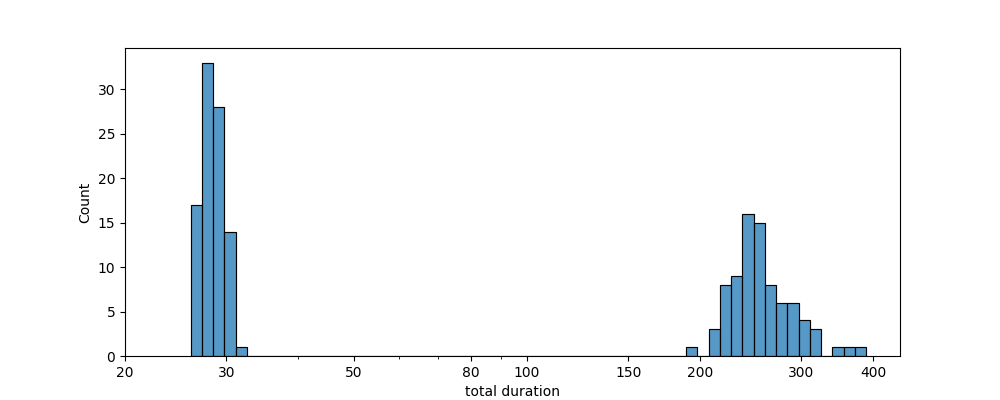
\includegraphics[width=8.5cm]{img/lambda_total_durations.png}
      \caption{ distribution of the total duration of the function. Note that the x axis is log scale }
    \label{fig:lambda-total-durations}
\end{figure}

However, only few web servers actually run entirely on serverless offerings
today. There are many reasons that developers choose not to use serverless,
despite in theory having workloads that are well-suited for the serverless
environment~\cite{not-lambda-blog,reddit-serverless2}. Popular complaints
include provider lock in, lack of insight for debugging and telemetry, and
variable runtimes.


We focus on what is arguably the most fundamental of these complaints; which is
the variable runtimes. We run a small experiment with a hello world style lambda
function that simply sleeps for 20ms and then returns. We use AWS
Xray~\cite{aws-xray} to measure its latency, with incovations spaced randomly
between 0 and 10 minutes. The results are in
Figure~\ref{fig:lambda-total-durations}. The times on the left side of the graph
are clearly the execution times from warm start, which remain somewhat stable.
The reason for this is likely that AWS is able to simply route the new request
to the machine with the existing container on it. The right grouping in the
graph is then the invocations that hit cold starts, whose overall latencies vary
between 200 and 400ms, meaning that when a request encounters cold start, the
variance in observed latency goes up a lot. 

\begin{figure}[t!]
  \centering
    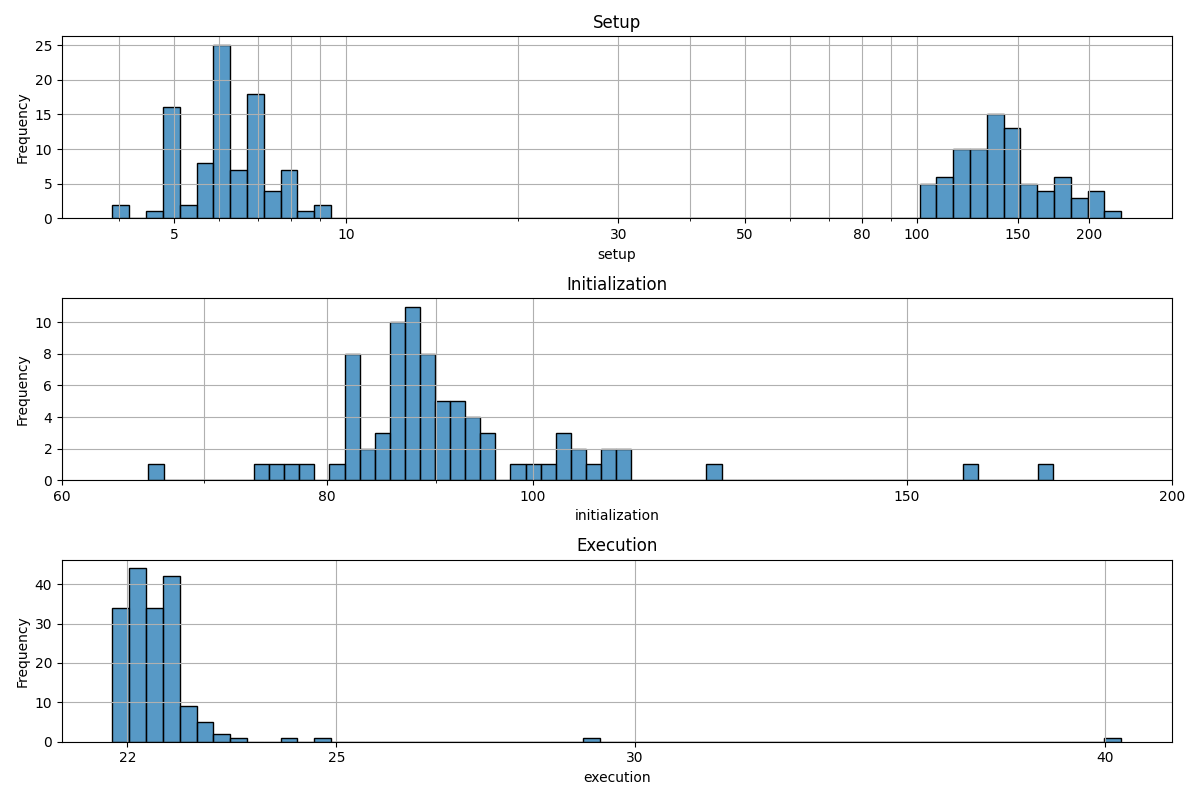
\includegraphics[width=8.5cm]{img/lambda_duration_breakdown.png}
    \caption{ Breakdown of duration variation. Note that here too the x axes are all log scale }
  \label{fig:lambda-durations-breakdown}
\end{figure}

In order to better understand where that variability comes from, we look into a
breakdown of the latencies. We are able to break down the total duration into
three components: \textit{setup}, which includes placing the function and
creating the container; \textit{initialization}, which is any code that runs
before the function does, for example initializing the runtime, and any
extensions the function uses; and \textit{execution}, actually executing the
functions code. Xray only gives us the latter two values explicitly, we
calculate the setup time by looking at the total duration and subtracting the
initalization and execution times. 

We can see the resulting distributions in
Figure~\ref{fig:lambda-durations-breakdown}. The most stable component of the
duration is unremarkably the execution time, although with some outliers. The
initialization also has a fair amount of variance, although there are no
discernable groupings. The strongest variability, unsurprisingly, comes from the
setup portion. Here we can see the two groupings clearly: one on the right that
includes starting up the container, and one on the left that doesn't. The range
is larger on the right ($\sim$150ms) than it is on the left ($\sim$8ms). Where
exactly the latency here comes from is impossible to know without futher insight
into the system, but clear is that there is already a small variation in warm
start setting, where AWS doesn't even need to place a new container. And clear
is also that sometimes AWS is able to get the cold start container up and
running in just over 100ms, and sometimes it takes as much as $\sim$250ms.

\subsection{Approach}

Our approach addresses the variability of runtimes, which is undesirable for
latency sensitive jobs, by using \priceclass{}es as a metric to tell the
scheduler what to prioritize and what not. We will show that this allows us to
stabilize the runtimes for the high \class{} jobs. 

In fact, we use \class{}es to supplant completely the current interface, which
requires developers choose an amount of memory per function, which is then tied
to a cpu power (a potentially fractional amount of vCPUs). \Priceclass{}es are a
metric that has a number of benefits over resource reservations as an interface:
developers are more likely to have a good sense of it ahead of time, it is less
likely to be different across different invocations, it still gives the
scheduler the information it needs to decide what to schedule when, and finally
it more directly aligns the interests of the developer with those of the
provider by communicating on the level of what the provider and developer
actually care about: money, and latency (as achieved by \class{}es in the
system).


However, having \priceclass{}es also means that there are no clear guarantees
about what developers are getting when they put a price on a function they want
to run. In order to mitigate that somewhat and not go into bidding wars, we
propose exposing a fixed set of price classes. This is similar to how AWS has
different EC2 instance types, that are directly mapped to prices. Rather than
being a guarantee, the price class is instead a metric to express priority to
\sys{}, which it can then use to enforce a favoring of high class jobs.

